
\documentclass{beamer}


\mode<presentation>
{
  \usetheme{Hawke}
  \setbeamercovered{transparent}
}


\usepackage[english]{babel}
\usepackage[latin1]{inputenc}
\usepackage{times}
\usepackage[T1]{fontenc}
\usepackage{multimedia}


%%%%%%
% My Commands
%%%%%%

\newcommand{\ml}{{\sc matlab}}
\newcommand{\bb}{{\boldsymbol{b}}}
\newcommand{\bx}{{\boldsymbol{x}}}
\newcommand{\by}{{\boldsymbol{y}}}
\newcommand{\bfm}[1]{{\boldsymbol{#1}}}

%%%%

\title[Lecture 5] %
{Lecture 5 - Iterative Methods}


\author[I. Hawke]{I.~Hawke}

\institute[University of Southampton]%
{
  School of Mathematics, \\
  University of Southampton, UK
}

\date[Semester 1]{MATH3018/6141, Semester 1}

\subject{Numerical methods}

\pgfdeclareimage[height=0.5cm]{university-logo}{mathematics_7469}
\logo{\pgfuseimage{university-logo}}

\AtBeginSection[]
{
  \begin{frame}<beamer>
    \frametitle{Outline}
    \tableofcontents[currentsection]
  \end{frame}
}



\begin{document}

\begin{frame}
  \titlepage
\end{frame}

\section{Iterative Methods}

\subsection{Iterative Methods}

\begin{frame}
  \frametitle{Iterative Methods}

   We (still) want to solve the linear system
   \begin{equation*}
     A \bx = \bb.
   \end{equation*}
   All direct methods require ${\cal O}(n^3)$ operations. For large
   matrices this takes time and each operation introduces error that
   may accumulate. Other methods may be preferable. \pause

   \vspace{1ex}

   Iterative methods build a \emph{sequence} of approximate
   solutions. Start from ``guess'' $\bx^{(0)}$ and compute
   approximations $\bx^{(1)}, \bx^{(2)}, \dots, \bx^{(N)}$ which
   converge to the exact solution.

   \vspace{1ex}

   Sequence can be truncated to save time or when solution found to
   sufficient accuracy. \pause

   \vspace{1ex}

   Key elements of an iterative method:
   \begin{enumerate}
   \item A rapid convergence to the correct solution,
   \item A fast algorithm for computing each successive approximation.
   \end{enumerate}

\end{frame}

\begin{frame}
  \frametitle{A general framework}

  Standard ``notation'' is to split the matrix as
  \begin{equation*}
    A = N - P,
  \end{equation*}
  where $N$ and $P$ are (as yet unknown) $n \times n$ matrices.
  The linear system becomes
  \begin{equation*}
    N \bx = P \bx + \bb.
  \end{equation*} \pause

  Then \emph{assume} that we have an approximate solution, or guess,
  $\bx^{(0)}$, and define the sequence
  \begin{equation*}
    N \bx^{(i)} = P \bx^{(i - 1)} + \bb, \quad i = 1, 2, \dots
  \end{equation*} \pause

  Obviously consistent with the original equation.  The algorithm will
  only be useful if
  \begin{enumerate}
  \item $N$ is nonsingular, and
  \item The linear system $N \bfm{y} = \bfm{z}$ is ``easy'' to solve.
  \end{enumerate}

\end{frame}


\subsection{Jacobi's Method}

\begin{frame}
  \frametitle{General assumptions}

  \vspace{2ex}

  In what follows we shall always assume that all diagonal entries are
  1. \pause

  \vspace{2ex}

  If this is not true, we can always arrange it to be so by dividing
  each row by its diagonal element. \pause

  \vspace{2ex}

  If the diagonal element of any row is zero, permute the rows. It
  must be possible to arrange a \emph{nonsingular} matrix such that
  every diagonal element is non-zero just by row operations.

\end{frame}

\begin{frame}
  \frametitle{Jacobi's Method}

  One key requirement on the split
  \begin{equation*}
    A = N - P
  \end{equation*}
  was that the $N \bfm{y} = \bfm{z}$ should be easy to solve. The
  simplest possible problem would be $N = I$. \pause

  \vspace{1ex}

  This means (as $A$ is 1 on the diagonal) that
  \begin{equation*}
    P = A_L + A_U
  \end{equation*}
  where $A_L$ and $A_U$ are the ``triangular'' parts of $-A$ (note
  sign!). The iteration scheme is
  \begin{equation*}
    \bx^{(i)} =  (A_L + A_U) \bx^{(i - 1)} + \bb, \quad i = 1, 2, \dots
  \end{equation*}
  and the convergence matrix is $M = P$.

\end{frame}

\begin{frame}
  \frametitle{Example of Jacobi's Method}

  We look at the solution of the simple linear system
  \begin{equation*}
    \begin{pmatrix}
      3 & 1 \\
      1 & 3
    \end{pmatrix}
    \begin{pmatrix}
      x_1 \\ x_2
    \end{pmatrix} =
    \begin{pmatrix}
      5 \\ 7
    \end{pmatrix}
  \end{equation*}
  using Jacobi's Method. \pause  Ensure the diagonal
  elements are all 1:
  \begin{equation*}
    A =
    \begin{pmatrix}
      1 & \tfrac{1}{3} \\
      \tfrac{1}{3} & 1 \\
    \end{pmatrix},
    \quad \bb =
    \begin{pmatrix}
      \tfrac{5}{3} \\ \tfrac{7}{3}
    \end{pmatrix}.
  \end{equation*} \pause
  Check convergence by computing
  \begin{equation*}
    M = P =
    \begin{pmatrix}
      0 & -\tfrac{1}{3} \\
      -\tfrac{1}{3} & 0
    \end{pmatrix}
  \end{equation*}
  which implies, as $\varrho(M) = 1 / 3 < 1$, that the method will
  converge.

\end{frame}

\begin{frame}
  \frametitle{Example of Jacobi's Method 2}

  \begin{columns}
    \begin{column}{0.475\textwidth}
      The sequence has entries
      \begin{tabular}{|c|c c|}
        $i$ & $x_1$ & $x_2$ \\ \hline
        $0$ & $0$ & $0$ \\
        $1$ & $5 / 3$ & $7 / 3$ \\
        $2$ & $0.888889$ & $1.777778$ \\
        $5$ & $1.008230$ & $2.004115$ \\
        $10$ & $0.999983$ & $1.999966$ \\
        $100$ & $1.000000$ & $2.000000$
      \end{tabular}
    \end{column}
    \begin{column}{0.525\textwidth}
      \begin{center}
        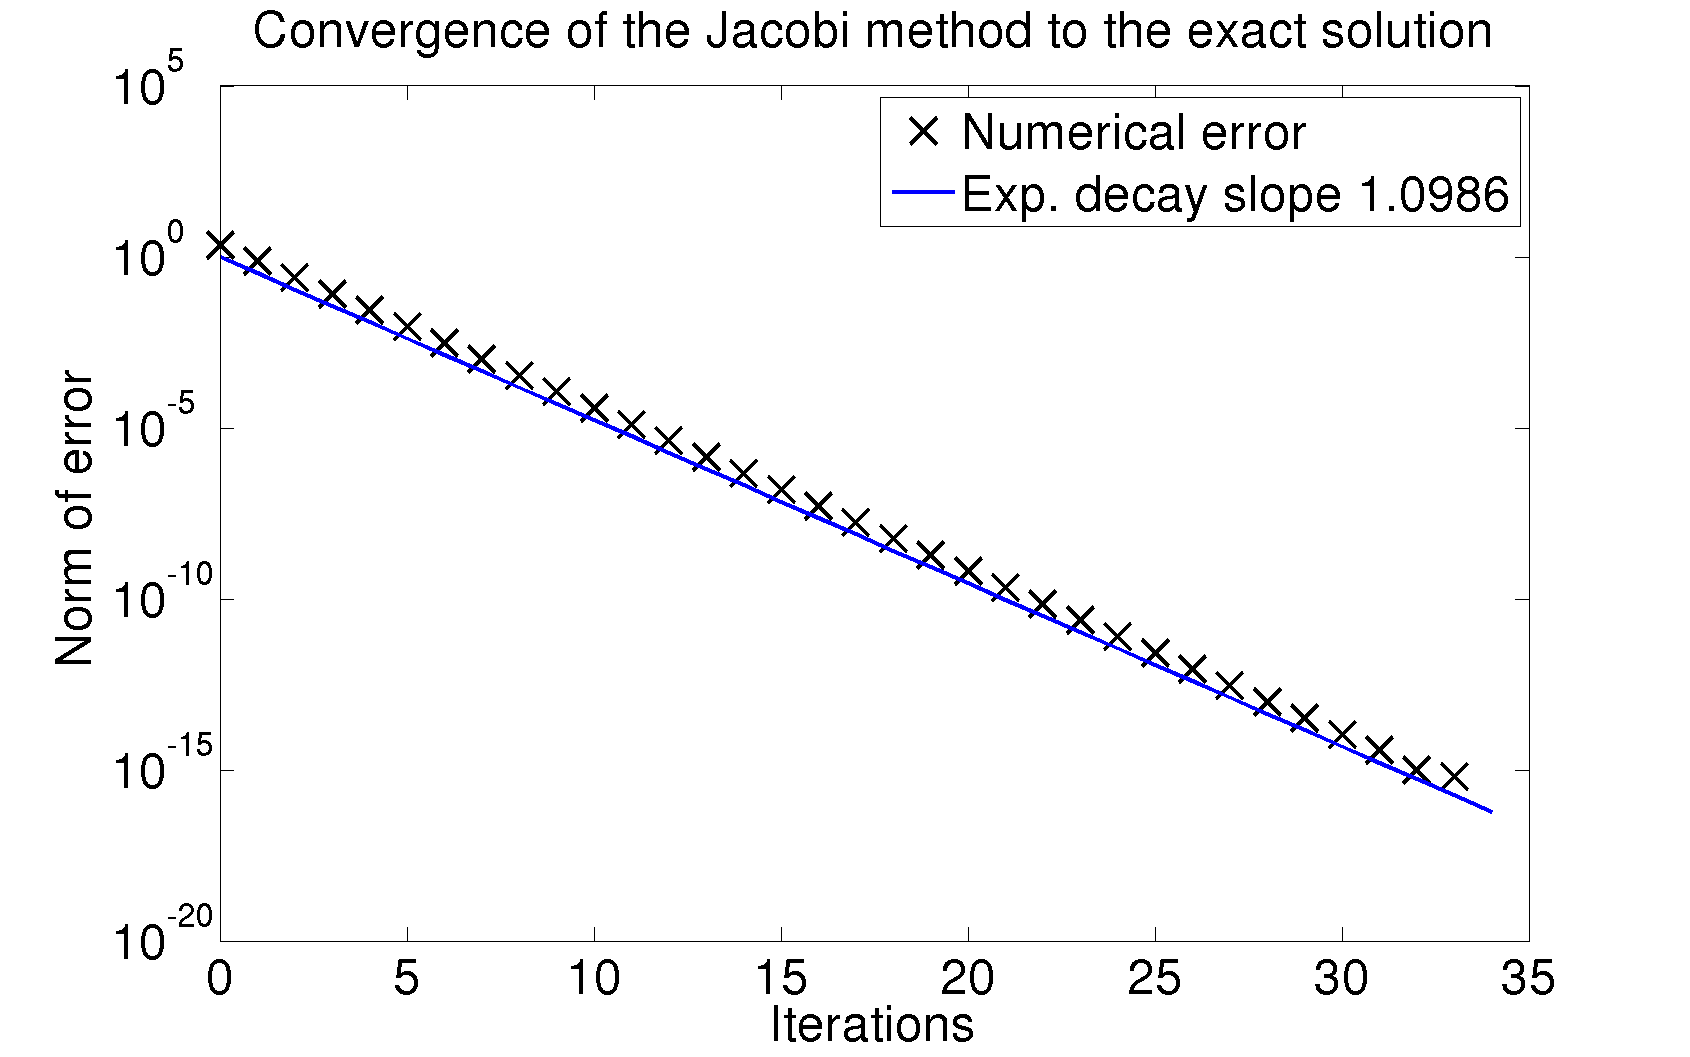
\includegraphics[width=\textwidth]{figures/Jacobi1}
      \end{center}
    \end{column}
  \end{columns}

  \vspace{1ex}

  A starting ``guess'' of $\bx = \bfm{0}$ appears to converge to $\bx
  = (1, 2)^T$. The convergence is exponential with a slope $\sim 1$.

\end{frame}


\subsection{Convergence}

\begin{frame}
  \frametitle{Convergence}

  To work, the sequence
  \begin{equation*}
    \bx^{(i)} = N^{-1} \left( P \bx^{(i - 1)} + \bb \right), \quad i =
    1, 2, \dots
  \end{equation*}
  must have a limit.  Intuitively clear that the matrix $M =
  N^{-1} P$ is central to the convergence or otherwise of
  this sequence.

  \vspace{1ex}

  {\bf Theorem}: The iterative method described converges if and only
  if $M = N^{-1} P$ exists and
  \begin{equation*}
    \varrho (M) \equiv \max_i | \lambda_i | < 1.
  \end{equation*}

  \begin{overlayarea}{\textwidth}{0.3\textheight}
    \only<2|handout:0>
    {
      View $\bx^{(i)}$ as a vector in $n$-dimensional space: ensures
      that repeatedly multiplying by $M$ does not cause result to
      diverge.
    }
    \only<3>
    {
      The \emph{spectral radius} $\varrho (M)$ can be hard
      to compute. Often use the weaker condition
      \begin{equation*}
        \| M \| < 1 \Rightarrow \text{Method converges}.
      \end{equation*}
    }
  \end{overlayarea}

\end{frame}


\section{Summary}

\subsection{Summary}

\begin{frame}
  \frametitle{Summary}

  \begin{itemize}
  \item Iterative methods are often based on the split
    \begin{equation*}
      A = N - P.
    \end{equation*}
  \item Convergence depends on $M = N^{-1}P$.
  \item Jacobi chooses $N = I$ and converges slowly.
  \end{itemize}

\end{frame}

\end{document}



%%% Local Variables:
%%% mode: latex
%%% TeX-master: t
%%% End:
